\documentclass{beamer}
\usepackage{cancel, algpseudocode, hyperref, tikz, venndiagram, centernot}

\title{CS 70 Discussion 6B}
\date{October 11, 2024}

\begin{document}

\frame{\titlepage}

\begin{frame}
    \frametitle{Counting}
    Some facts that always hold:
    \begin{itemize}
        \item Symmetry: $\binom{n}{k}=\binom{n}{n-k}$
        \item Summation: $2^n=\sum_{i=0}^n\binom{n}{i}$
        \item Recursive Definition: $\binom{n}{k}=\binom{n-1}{k}+\binom{n-1}{k-1}$
        \item Binomial Theorem: $(a+b)^n=\sum_{i=0}^n\binom{n}{i}a^ib^{n-i}$
    \end{itemize}
    You can use Pascal's triangle to get binomial coefficients quickly. The row represents $n$, the column represents $k$, and $\binom{n}{k}$ is the value. The rows and columns are $0$-based indexed (the first row and column are $0$, not $1$):
    \begin{center}
        \includegraphics[scale=0.15]{Images/pascal-triangle.png}
    \end{center}

\end{frame}

\begin{frame}
    \frametitle{Principle of Inclusion-Exclusion}
    {\bf Problem}: I want to count the number of elements in the set $A_1\cup A_2\cup...\cup A_n$.\\
    {\bf Solution}: For the $n=2$ case:\\
    \begin{center}
        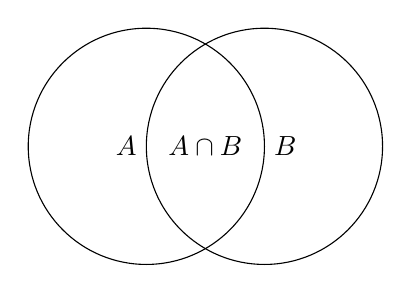
\begin{tikzpicture}
            \draw[] (0,0) circle (1.5cm) node[left] {$A$};
            \draw[] (1.5,0) circle (1.5cm) node[right] {$B$};
            \node at (0.75,0) {$A \cap B$};
        \end{tikzpicture}
    \end{center}
    We have $|A\cup B|=|A|+|B|-|A\cap B|$. But, general formula is:
    \begin{gather*}
        \left|\bigcup_{i=1}^n A_i\right|=\sum_{s=1}^n(-1)^{s-1}\sum_{\substack{S\subseteq\{1,2,...,n\}\\|S|=s}}\left|\bigcap_{i\in S}A_i\right|
    \end{gather*}
\end{frame}

\begin{frame}
    \frametitle{Combinatorial Proofs}
    These are essentially informal proofs where you prove that two sets are the same size by setting-up a ``story'' where counting the elements in one set is functionally equivalent to counting the elements in the other set. Example for proving $\binom{n}{k}=\binom{n}{n-k}$:
    \begin{itemize}
        \item Left-Hand Side (LHS): We have $n$ people. We want to pick $k$ people out of these $n$ people to be representatives. Thus $\binom{n}{k}$.
        \item Right-Hand Side (RHS): We have $n$ people. We pick $n-k$ people to {\it not} be representatives, and we make the rest of the $k$ people representatives. Thus $\binom{n}{n-k}$.
    \end{itemize}
    Both these situations finds all possible groups of $k$ representatives.
\end{frame}

\begin{frame}
    \frametitle{Countability}
    We define three main types of sets:
    \begin{itemize}
        \item {\bf Finite-Sized, Countable Set}: A set with a finite number of elements
        \begin{itemize}
            \item Examples: any set with a finite size (ex. $\{0.342,5554,\frac{1}{4}\}$)
        \end{itemize}
        \item {\bf Infinite-Sized, Countable Set}: A set with an infinite number of elements, but you can {\it order} all of the elements (i.e. you can create an infinite-length list of all elements in the set and each element has an index)
        \begin{itemize}
            \item Examples: $\mathbb{N},\mathbb{Z},\mathbb{Q}$
        \end{itemize}
        \item {\bf Infinite-Sized, Uncountable Set}: A set where there is no way to order the elements of the set.
        \begin{itemize}
            \item Examples: $\mathbb{R},\mathbb{C}$
        \end{itemize}
    \end{itemize}
    {\bf Cardinality}/Size Comparison: $|\text{Finite-Sized, Countable Set}|<|\text{Infinite-Sized, Countable Set}|<|\text{Infinite-Sized, Uncountable Set}|$
\end{frame}

\begin{frame}
    \frametitle{Countability (Cont.)}
    {\bf Problem}: How to prove a set $S$ is countable?\\
    {\bf Solution}: Here are some options:
    \begin{itemize}
        \item Prove that there is some function $f:S\rightarrow\mathbb{N}$ that is one-to-one (injective), which proves $|S|\leq|\mathbb{N}|$.
        \item Prove that there is some bijective function $f:S\rightarrow\mathbb{N}$ (one-to-one and onto), which proves $|S|=|\mathbb{N}|$ ($S$ is an infinite-sized, countable set).
        \item Prove that there are some one-to-one functions $f:S\rightarrow\mathbb{N}$ and $g:\mathbb{N}\rightarrow S$, which proves $|S|=|\mathbb{N}|$ (this is another way to prove a bijection between $S$ and $\mathbb{N}$).
        \item Prove that $S\subseteq T$, where you already know $T$ is countable.
    \end{itemize}
\end{frame}

\begin{frame}
    \frametitle{Countability (Cont.)}
    {\bf Problem}: How to prove a set $S$ is uncountable?\\
    {\bf Solution}: Here are some options:
    \begin{itemize}
        \item Prove that $S\supseteq T$, where $T$ is some uncountably infinite set.
        \item Use a {\bf Cantor's Diagonalization} proof.
    \end{itemize}
\end{frame}

\begin{frame}
    \frametitle{Cantor's Diagonalization}
    Proof technique:
    \begin{enumerate}
        \item Assume that set $S$ is countable.
        \item This means that all elements can be ordered. Example for $S=[0,1]$:
        \begin{align*}
            &0.0234562374533564\dots\\
            &0.6547345765765462\dots\\
            &\vdots
        \end{align*}
        \item Create a new element $x\in S$ by changing the diagonal elements of our table. Example: for $S=[0,1]$, we can turn all non-$5$ digits into $5$s and all $5$-digits into $2$s along the diagonal:
        \begin{align*}
            x=0.525525...
        \end{align*}
        \item $x\in S$, but it cannot be in our table. Contradiction!
    \end{enumerate}
\end{frame}

\end{document}
